\chapter{Background}
\section{Twisted Moir\'e Physics}
\subsection{Transition Metal Dichalcogenides}
Graphene, as the most famous 2D materials first discovered in 2004 by Geim and Novoselov \cite{novoselov2004electric}, is well-known for the presence of Dirac points in its band structure.

% For the honeycomb lattice constituted of carbon atoms only, there exists sublattice (inversion) symmetry between $A,B$ sites. For spinless electrons, where Hamiltonian is written in such pseudospin basis as a general two-by-two matrix $H(\bm k)=\bm d(\bm k)\cdot\bm \tau$ with real vector coefficients $\bm d(\bm k)$, the inversion operator $\mathcal P$ exchanging $A,B$ sites can be represented as $P=\tau_x$. Graphene also possesses time-reversal symmetry, and for spinless electrons the time-reversal operator is simply a complex conjugate $T=K$. Therefore, the combination of inversion symmetry and time-reversal symmetry keeping the momentum unchanged: $\mathcal P\mathcal T:\bm k\mapsto\bm k$, requires the Hamiltonian to satisfy
% \begin{equation*}
%     \tau_x^{-1}H^*(\bm k)\tau_x=H(\bm k),
% \end{equation*}
% implying $d_3(\bm k)=0$ or $H(\bm k)=d_1(\bm k)\tau_x+d_2(\bm k)\tau_y$ with ALL matrix element off-diagonal. Now because both the momentum and the Hamiltonian share the same dimensionality, given one zero solution of the eigen equation $\det|\lambda I-H(\bm k)|=0$, any perturbation preserving the inversion and time-reversal symmetries, i.e., constituted of $\tau_x$ and $\tau_y$ matrices, cannot destroy such zero point. That is the typical example of symmetry-protected Dirac points (if exists) in graphene.

% To obtain the low-energy description of graphene, we can implement the spatial $C_3$ rotation symmetry to the Hamiltonian
% \begin{equation}\label{eq:C3 rotation constraint}
%     C_3^{-1}H(\bm k)C_3=H(\mathcal C_3^{-1}\bm k).
% \end{equation}
% \noindent Precisely speaking, we can expand the general Hamiltonian around $K$ and $K'$ to the lowest linear-order
% \begin{equation*}
%     d_1(\bm k)=a_{10}+a_{11}k_x+a_{12}k_y,\quad d_2(\bm k)=a_{20}+a_{21}k_x+a_{22}k_y
% \end{equation*}
% % or
% % \begin{equation*}
% %     H(\bm k)=\begin{pmatrix}
% %                                                                  & (a_{10}-ia_{20})+(a_{11}-ia_{21})k_x+(a_{12}-ia_{22})k_y \\
% %         (a_{10}+ia_{20})+(a_{11}+ia_{21})k_x+(a_{12}+ia_{22})k_y &
% %     \end{pmatrix}
% % \end{equation*}
% and insert back to the constraint Eq. \eqref{eq:C3 rotation constraint}. One gets
% \begin{equation*}
%     a_{31}=a_{32}=0,\quad a_{10}=a_{20}=0,\quad a_{12}=-a_{21},\quad a_{11}=a_{22},
% \end{equation*}
% and we end up with the well-known Dirac cone Hamiltonian
\begin{equation}
    H_K(\bm k)=\hbar v_F\bm k\cdot\bm\tau\equiv\hbar v_F|\bm k|\left(\begin{array}{cc}
                      & e^{-i\theta_k} \\
        e^{i\theta_k} &
    \end{array}\right)
\end{equation}
with the angle of the momentum $\theta_k\equiv\arctan\frac{k_y}{k_x}$.


Transition metal dichalcogenides (TMDs) of chemical formula MX$_2$, on ther other hand, has a more complicated structure comprising a plane having hexagonally-placed transition metal atoms M (group-IIIB to group-IIB) placed between two chalcogen atom-based hexagonal planes X (e.g., S, Se, Te). There are three monolayer structures: the \emph{trigonal prismatic} 1H phase, the \emph{distorted octahedral} 1T phase, and the \emph{dimerized} 1T' phase, as are shown in Fig. \ref{fig:TMD_electonic_properties}.
\begin{figure}[!htp]
    \centering
    \includegraphics[width=1.0\textwidth]{figures/Background/TMD.png}
    \caption{\textbf{Structure and electronic properties of TMDs} adapted from Ref. \cite{manzeli20172d}. \textbf{(a)} Atomic structure of single layers of TMD in their \emph{trigonal prismatic} (2H), \emph{distorted octahedral} (1T) and \emph{dimerized} (1T') phases. \textbf{(b)} ``Periodic table'' of known layered TMDs, organized based on the transition metal elements, their existing structural phases (2H, 1T and 1T'), and the observed electronic phases (see the right panel). \textbf{(c)} Evolution of the band structure of 2H-MoS$_2$ from bulk material down to monolayers. Clearly a indirect gap to direct gap transition occurs for monolayer material only. \textbf{(d)} Schematic band structure of 2H-MoS$_2$, showing the spin splitting (orange and blue colors) at K and K' points.)}
    \label{fig:TMD_electonic_properties}
\end{figure}
We will mostly focus on the group V and group VI transition metal elements, particularly those with 1T and 1T' phases shown to be unstable. So without loss of generalization, when we talk about monolayer TMDs in this thesis, we always refer to the 1H phase structure.

For monolayer TMDs of 1H phase, the corresponding bulk material are mostly of 2H stacking form, with \emph{alternating} alignment of transition metal atoms and chalcogen atoms, as is shown in (a) in Fig. \ref{fig:MoS2_Di}.
\begin{figure}[!htp]
    \centering
    \includegraphics[width=0.8\textwidth]{figures/Background/MoS2_Di.png}
    \caption{\textbf{MoS$_2$ Crystal Structure and Band Structure} adapted from Ref. \cite{xiao2012coupled}. \textbf{(a)} The unit cell of bulk 2H-MoS$_2$. \textbf{(b)} Top view of MoS$_2$ monolayer. \textbf{(c)} Schematic drawing of the band structure at the band edges located at the K points.}
    \label{fig:MoS2_Di}
\end{figure}
Experimentally, there has been reports on the emergence of the peak in the optical spectroscopy study in Ref. \cite{mak2010atomically} and photoluminescence (PL) signals in Ref. \cite{splendiani2010emerging}, which is ascribed as the manifestation on the evolution of of the TMD band structure from bulk's indirect gap to monolayer's direct $K$-$K$ gaps, see (c) in Fig. \ref{fig:TMD_electonic_properties}.

Taking group-IV dichalcogenides MX$_2$ as the example, the 2H stacking bulk material has space group $D_{6h}$ with inversion symmetry (see (a) in Fig. \ref{fig:MoS2_Di}), but reduces to $D_{3h}$ breaking the inversion symmetry down to monolayers. For monolayer MX$_2$, DFT calculation tells that the relevant orbitals within the conduction and valence bands around $K$ and $K'$ points are mostly from d-orbitals \cite{mattheiss1973band}. From the character table of $D_{3h}$ (see, for example, \url{http://symmetry.jacobs-university.de/cgi-bin/group.cgi?group=603&option=4}), we know that the trigonal prismatic crystal field splits the d-orbitals of transition metal elements into three groups: $A_1'(d_{z^2})$, $E'(d_{xy}, d_{x^2-y^2})$, and $E''(d_{xz}, d_{yz})$, where the former two groups $A_1'$ and $E'$ is even under the in-plane mirror symmetry $\sigma_h: z\rightarrow-z$, while the latter one $E''$ is odd under $\sigma_h$. Now that only two bands are concerned in our analaysis: the conduction band and the valence band, we can simply take the irreps $A_1'$ and $E'$ into account, resulting in a simple two-band model $H_\tau(\bm k)=\bm d(\bm k)\cdot\bm\sigma$ if the spin-orbit coupling is temporarily ignored.

To the lowest-order expansion, the constant part of the diagonal terms represent the $K$-$K$ (or $K'$-$K'$) direct band gap $\Delta$. While for the off-diagonal term, we can either use the brute-force expansion and fix the expansion coefficients using $C_3$ rotation transformation as we did for graphene, or use the standard $\bm k\cdot\bm p$ analysis \cite{dresselhaus1955spin,voon2009kp,kormanyos2015k} by computing the matrix element $\langle \psi_a|\frac{\hbar}{m}\bm k\cdot\hat{\bm p}|\psi_b\rangle$ for $|\psi_{a,b}\rangle\in\{|\psi_{A_1'}\rangle,|\psi_{E'}\rangle\}$. Note: not all terms survives in such matrix element. In fact, because we have the rotation eigenvalues $C_3|\psi_{A_1'}\rangle=|\psi_{A_1'}\rangle$ and $C_3|\psi_{E'}\rangle=e^{i\frac{2\pi}{3}}|\psi_{E'}\rangle$ (for $K$-valley, for example), and for $\hat p_\pm\equiv\hat p_x\pm i \hat p_y$ we have $C_3\hat p_\pm C_3^\dagger=e^{i\mp\frac{2\pi}{3}}$, the $C_3$ rotation tansformation forces either term within $H_{\bm k\cdot\bm p}\equiv\frac{\hbar}{2m}\bm k\cdot\hat{\bm p}\equiv\frac{\hbar}{2m}(k_+\hat p_- + k_-\hat p_+)$ to be vanishing in the off-diagonal matrix element, leaving simply the massive Dirac Hamiltonian (with insertion of valley index)
\begin{equation}
    H_{\text{eff}}^{\text{SOC off}}=H_0+H_{\bm k\cdot\bm p}=\begin{pmatrix}
        \frac{\Delta}{2} & Ak_-              \\
        Bk_+             & -\frac{\Delta}{2}
    \end{pmatrix}\equiv\hbar v_F(\tau k_x\sigma_x+k_y\sigma_y)+\frac{\Delta}{2}\sigma_z.
\end{equation}

Now let us include the spin-orbit couplings (SOC) in the $\bm k\cdot\bm p$ analaysis
\begin{equation*}
    H_{\bm k\cdot\bm\pi}\equiv\frac{\hbar}{m}\bm k\cdot\left(\bm p+\frac{\hbar}{4mc^2}\bm s\times\nabla V\right).
\end{equation*}
The SOC Hamiltonian can also be written as $H_{\text{SOC}}=\lambda\bm L\cdot\bm  s=\lambda(L_z s_z + L_+  s_- + L_-  s_+)$. Noting that both $L_+$ and $L_-$ are odd under in-plane mirror symmetry $\sigma_h$, while $L_z$ is even, so the orbital-part of the matrix element satisfying $\langle\psi_a|L_\pm|\psi_b\rangle\equiv\langle\psi_a| s_h^{-1}  s_h L_\pm s_h^{-1} s_h|\psi_b\rangle$ must connect states whose orbital contents behaves \emph{differently} under $\sigma_h$. However, our chosen basis $|\psi_{A_1'}\rangle$ and $|\psi_{E'}\rangle$ are both even under $\sigma_h$, so we are left with simply the $L_z$ term, resulting
\begin{equation}
    H_{\text{eff}}=H_0+H_{\bm k\cdot\bm\pi}=H_{\text{eff}}^{\text{SOC off}}\otimes s_0 + \begin{pmatrix}
        \Delta_{A_1'\text{-SOC}} &                        \\
                                 & \Delta_{E'\text{-SOC}}
    \end{pmatrix}\otimes s_z
\end{equation}
with $\Delta_{A_1'\text{-SOC}}$ and $\Delta_{E'\text{-SOC}}$ dictating the band splittings due to SOC. The energy scale of them can be read from the DFT results in Fig. \ref{fig:monolayer_TMD_band_structure},
\begin{figure}[!htp]
    \centering
    \includegraphics[width=0.9\textwidth]{figures/Background/monolayer_TMD_band_structure.png}
    \caption{\textbf{DFT Band Structures for Several MX$_2$ Monolayer Materials} (extracted from \cite{ramasubramaniam2012large}).}
    \label{fig:monolayer_TMD_band_structure}
\end{figure}
where $\Delta_{A_1'\text{-SOC}}$ always turns out to be almost vanishing so we jut ignore it. The final form of the effective Hamiltonian (with insertion of valley index)
\begin{equation}\label{eq:MoS2 kdotp}
    H_{\text{eff}}=\bigg(\hbar v_F(\tau k_x\sigma_x+k_y\sigma_y)+\frac{\Delta}{2}\sigma_z\bigg)\otimes s_0 - \lambda\tau\frac{\sigma_z-\mathbf 1}{2}\otimes s_z.
\end{equation}

\subsection{Moir\'e Continuum Hamiltonian}
Moir\'e patterns are known as the interference patterns generated when two or more periodic structures of the same scale (lattice constant $a$) are overlaid. The interference pattern exhibits a new large-scale (coin as \emph{Moir\'{e} scale}) periodic structure on top of the original one (which can be different from the original ones), so that the original lattice information is smeared out, leaving physics occurring at such new Moir\'{e} scale.

The general bilayer system can be described with two set of grids spanned by $\{\bm R_{l,1},\bm R_{l,2}\}$ with $l=1,2$ labeling the layers. We are interested in the physics when the two layers are related with some rotation $\mathcal R_\theta$  and some displacement $\bm d$. Namely the same cartesian coordinate within these two coordinates systems are related with the linear transformation: $\bm{r}_{l',\alpha}=\mathcal R_\theta\bm{r}_{l,\alpha}+\bm d$. This leads to to a useful identity for the inner product that
\begin{equation}\label{eq:twisted dot product}
    \bm k_{l'}\cdot\bm r_{l',\alpha}\equiv(\mathcal R_\theta\bm k_l)\cdot(\mathcal R_\theta\bm r_{l,\alpha}+\bm d)\equiv\bm k_l\cdot\bm r_{l,\alpha}+\bm k_l\cdot\bm d,
\end{equation}
where we recognize $\bm k_l\equiv\mathcal R_\theta\bm k_{l'}$.

Each layer possesses its own Bloch states
\begin{equation*}
    |\bm k_l,\alpha\rangle =\dfrac{1}{\sqrt N}\sum_{\bm R_l} e^{i\bm k_l\cdot(\bm R_l+\bm\tau_{l,\alpha})}|\bm R_l+\bm\tau_{l,\alpha}\rangle,
\end{equation*}
so the general momentum-space Hamiltonian of the bilayer system can be obtained from the matrix element
\begin{align*}
    \langle\bm k_l,\alpha|H|\bm k'_{l'},\alpha'\rangle & =\frac{1}{N}\sum_{\bm R_l,\bm R'_{l'}}e^{-i\bm k_l\cdot(\bm R_l+\bm\tau_{l,\alpha})}e^{i\bm k'_{l'}\cdot(\bm R'_{l'}+\bm\tau_{l',\alpha'})}\langle\bm R_l+\bm\tau_{l,\alpha}|H|\bm R'_{l'}+\bm\tau_{l',\alpha'}\rangle.
\end{align*}
Since the Wannier center is highly localized in real-space, it is OK to take the real-space matrix element on the right hand side as a function of the distance of two Wannier centers only (and of course also labelled with the species of the Wannier orbitals), i.e.
\begin{equation*}
    \langle\bm R_l+\bm\tau_{l,\alpha}|H|\bm R'_{l'}+\bm\tau_{l',\alpha'}\rangle\simeq H_{l,\alpha;l',\alpha'}(\bm R_l+\bm\tau_{l,\alpha}-\bm R'_{l'}-\bm\tau_{l',\alpha'}),
\end{equation*}
which is know as the \emph{two-center approximation} \cite{bistritzer2011moire}. Scalar function $H(\bm R_l+\bm\tau_{l,\alpha}-\bm R'_{l'}-\bm\tau_{l',\alpha'})$ is still periodic. Switching to momentum space, and using the Poisson summation formula
\begin{equation*}
    \frac{1}{N}\sum_{\bm R}e^{i\bm R\cdot\bm q}=\sum_{\bm G}\mathcal F[e^{i\bm R\cdot\bm q}](\bm G)=\sum_{\bm G}\delta_{\bm q,\bm G}
\end{equation*}
we have
\begin{align}
    \langle\bm k_l,\alpha|H|\bm k'_{l'},\alpha'\rangle & =\frac{1}{N}\sum_{\bm R_l,\bm R'_{l'}}e^{-i\bm k\cdot(\bm R_l+\bm\tau_{l,\alpha})}e^{i\bm k'_{l'}\cdot(\bm R'_{l'}+\bm\tau_{l',\alpha'})}\frac{1}{NA}\sum_{\bm q}e^{i\bm q\cdot(\bm R_l+\bm\tau_{l,\alpha}-\bm R'_{l'}-\bm\tau_{l',\alpha'})}H_{l,\alpha;l',\alpha'}(\bm q)                  \nonumber                    \\
                                                       & = \frac{1}{A}\sum_{\bm q}\left(\dfrac{1}{N}\sum_{\bm R_l}e^{i\bm R_l\cdot(\bm q-\bm k_l)}\right)\left(\dfrac{1}{N}\sum_{\bm R'_{l'}}e^{i\bm R'_{l'}\cdot(\bm q-\bm k'_{l'})}\right)e^{i\bm\tau_{l,\alpha}\cdot(\bm q-\bm k_l)} e^{-i\bm\tau_{l',\alpha'}\cdot(\bm q-\bm k'_{l'})}H_{l,\alpha;l',\alpha'}(\bm q) \nonumber \\
                                                       & =\frac{1}{A}\sum_{\bm q}\sum_{\bm G_l,\bm G_{l'}}\delta_{\bm q-\bm k_l,\bm G_l}\delta_{\bm q-\bm k'_{l'},\bm G_{l'}}e^{i\bm\tau_{l,\alpha}\cdot(\bm q-\bm k_l)} e^{-i\bm\tau_{l',\alpha'}\cdot(\bm q-\bm k'_{l'})}H_{l,\alpha;l',\alpha'}(\bm q)                                         \nonumber                        \\
                                                       & = \frac{1}{A}\sum_{\bm G_l,\bm G_{l'}}\delta_{\bm k_l+\bm G_l,\bm k'_{l'}+\bm G_{l'}} e^{i\bm\tau_{l,\alpha}\cdot\bm G_l}e^{-i\bm\tau_{l',\alpha'}\cdot\bm G_{l'}}H_{l,\alpha;l',\alpha'}(\bm k_l+\bm G_l)\nonumber                                                                                                       \\
                                                       & = \frac{1}{A}\sum_{\bm G_l,\bm G_{l'}}\delta_{\bm k_l+\bm G_l,\bm k'_{l'}+\bm G_{l'}} e^{i\bm G_l\cdot(\bm\tau_{l,\alpha}-\bm\tau_{l,\alpha'})}e^{-i\bm G_l\cdot\bm d} H_{l,\alpha;l',\alpha'}(\bm k_l+\bm G_l),\label{eq:two-center_approximation}
\end{align}
where we use the fact that the two layers shares the same value of $\bm G$ but differ by at most some rotations, and the linear transformation Eq.\eqref{eq:twisted dot product}.

The momentum-space expression Eq. \eqref{eq:two-center_approximation} is the general result of the two-center approximation. It is true for both intralyer hopping processes and interlayer tunneling processes. The Dirac delta function signatures the momentum convervation of the hopping/tunneling processes within/across top and bottom layers. And the exponential $e^{-i\bm G_l\cdot\bm d}$ signatures the stacking dependence ($\bm d=0$ for AA stacking). It turns out to be more helpful to explicitly split Eq.\eqref{eq:two-center_approximation} into intralayer and interlayer parts:
\begin{align}
    \langle \bm k_l,\alpha|H|\bm k'_{l'},\alpha'\rangle & = \delta_{l,l'}\dfrac{1}{A}\bigg[\sum_{\bm G_l}\delta_{\bm k_l,\bm k'_{l'}}H_{l,\alpha;l',\alpha'}(\bm k_l+\bm G_l)e^{-i\bm G_l\cdot\bm d}\bigg]\nonumber                                                                                                                                   \\
                                                        & \quad +(1-\delta_{l,l'})\dfrac{1}{A}\bigg[\sum_{\bm G_l,\bm G_{l'}}\delta_{\bm k_l+\bm G_l,\bm k'_{l'}+\bm G_{l'}}H_{l,\alpha;l',\alpha'}(\bm k_l+\bm G_l) e^{i\bm G_l\cdot(\bm\tau_{l,\alpha}-\bm\tau_{l,\alpha'})}e^{-i\bm G_l\cdot\bm d}\bigg]\nonumber                                  \\
                                                        & \equiv\delta_{l,l'}\delta_{\bm k_l,\bm k'_{l'}}\dfrac{1}{A}\bigg[H_{l,\alpha;l',\alpha'}(\bm k_l) + \sum_{\bm G_l\neq0}H_{l,\alpha;l',\alpha'}(\bm k_l+\bm G_l)e^{-i\bm G_l\cdot\bm d}\bigg]\nonumber                                                                                       \\
                                                        & \quad +(1-\delta_{l,l'})\dfrac{1}{A}\bigg[\sum_{\bm G_l,\bm G_{l'}}\delta_{\bm k_l+\bm G_l,\bm k'_{l'}+\bm G_{l'}}H_{l,\alpha;l',\alpha'}(\bm k_l+\bm G_l) e^{i\bm G_l\cdot(\bm\tau_{l,\alpha}-\bm\tau_{l,\alpha'})}e^{-i\bm G_l\cdot\bm d}\bigg],\label{eq:two-center_approximation_split}
\end{align}
where we explicitly separate out the $\bm G_l=0$ and $\bm G_l\neq0$ term in Eq.\eqref{eq:two-center_approximation_split}, as is suggested in Ref. \cite{jung2014ab}. Clearly only the $\bm G_l=0$ parts of the intralayer hoppings are diagonal in the original Bloch basis, while the $\bm G_l\neq0$ part of both the intralayer hoppings and the interlayer tunnelings contribute to the off-diagonal terms. There are two kinds of summation in Eq.\eqref{eq:two-center_approximation_split}, $\sum_{\bm G_l}$ and $\sum_{\bm G_{l'}}$. Fortunately, both can be simplified from the following observations:

First of all, noting that we usuaully wish to derive the low-energy effective model for a small region of the BZ. For general discussion, let us denote such small region as $\bm{\mathcal K}_l$, and consider the perturbation around that region $\bm k_l=\bm{\mathcal K}_l+\delta\bm k_l$, then clearly we always have $|\delta\bm k_l-\delta\bm k_{l'}|\ll||\bm{\mathcal K}_l||$. On the other hand, the Dirac delta function in the interlayer tunneling term of Eq.\eqref{eq:two-center_approximation_split} tells that the only non-vanishing contributions are those satisfying $\delta\bm k_l-\delta\bm k_{l'}=\bm{\mathcal K}_l+\bm G_l-\bm{\mathcal K}_{l'}-\bm G_{l'}$. But clearly \textbf{most of the differences between the two collections $\{\bm{\mathcal K}_l+\bm G_l\}$ and $\{\bm{\mathcal K}_{l'}-\bm G_{l'}\}$ are no less than $||\text{BZ}||$, except for those when they differ by just a rotation --- this is reasonable because twisting angle $\theta$ appears as the only small parameter in our model setup}. As a consequence, the summation over $\bm G_{l'}$ is always associated with $\bm G_l$ and gets highly suppressed for those terms satisfying $\bm G_{l'}=\bm G_l$, resulting in a simple summation over $\bm G_l$ only.

Secondly, because the real-space profile $H_{l,\alpha;l',\alpha'}(\bm R_l+\bm\tau_{l,\alpha}-\bm R_{l'}-\bm\tau_{l',\alpha'})$ decays exponentially due to the locality of Wannier orbitals, the momentum-space profiles $H_{l,\alpha;l',\alpha'}(\bm k_l+\bm G_l)$ should also reflect such exponentially-decay behaviors. So \textbf{usuaully it is enough to keep only several low-order expansions for $\bm G_l$ in $H_{l,\alpha;l',\alpha'}(\bm k_l+\bm G_l)$ respecting the crystal symmetries}.


Depending on the position of the target region $\bm{\mathcal K}_l$, we are divided into two situations:
\begin{enumerate}
    \item If the target region $\bm{\mathcal K}_l$ is indeed close to some high-symmetry points at the zone boundary, like the $K$-point (or $K'$-point) in twisted bilayer graphene or twisted MoTe$_2$, and the small $M$-pocket of twisted monolayer FeSe, the collecion $\{\bm{\mathcal K}_l+\bm G_l\}$ will introduce other high-symmetry points with different crystal momentum compatible with rotation symmetries.

          If we denote $\bm q_1\equiv\bm{\mathcal K}_l-\bm{\mathcal K}_{l'}$, and introduce the other rotation-related crystal momentum differences as a finite set $\{\bm q_i\equiv C_n^{i-1}\bm q_1\}$, then Any momentum shift differences satisfying $\delta_{\delta\bm k_l-\delta\bm k'_{l'},\bm q_i}$ would contribute to the interlayer tunnelings. Consequently, the momentum-space Hamiltonian becomes
          \begin{align}
              \langle \bm k_l,\alpha|H|\bm k'_{l'},\alpha'\rangle & = \delta_{l,l'}\delta_{\bm k_l,\bm k'_{l'}}\frac{1}{A}\bigg[H_{l,\alpha;l',\alpha'}(\delta\bm k_l+\bm{\mathcal K}_l)+\sum_{\bm G_l}H_{l,\alpha;l',\alpha'}(\delta\bm k_l+\bm{\mathcal K}_l+\bm G_l)e^{-i\bm G_l\cdot\bm d}\bigg]                   \nonumber \\
                                                                  & +(1-\delta_{l,l'})\dfrac{1}{A}\bigg[\sum_i \delta_{\delta\bm k_l-\delta\bm k'_{l'},\bm q_i}H_{l,\alpha;l',\alpha'}(\delta\bm k_l+\bm{\mathcal K}_l+\bm G_l)e^{i\bm G_l\cdot(\bm\tau_{l,\alpha}-\bm\tau_{l',\alpha'})}e^{-i\bm G_l\cdot\bm d}\bigg] \nonumber \\
                                                                  & \simeq \delta_{l,l'}\delta_{\bm k_l,\bm k'_{l'}}\bigg[h^l_{\alpha\alpha'}(|\bm{\mathcal K}_l|)+\sum_{\bm G_l}V^l_{\alpha\alpha'}(|\bm{\mathcal K}_l|)e^{-i\bm G_l\cdot\bm d}\bigg]                                                                 \nonumber \\
                                                                  & \qquad+(1-\delta_{l,l'})\bigg[\sum_i \delta_{\delta\bm k_l-\delta\bm k'_{l'},\bm q_i}[T_i(\bm{\mathcal K}_l)]_{\alpha,\alpha'}\bigg],\label{eq:moire_Hamiltonian_at_high_symmetry_point}
          \end{align}
          where we recognize $H_{l,\alpha;l',\alpha'}(\delta\bm k_l+\bm{\mathcal K}_l+\bm G_l)\simeq H_{l,\alpha;l',\alpha'}(|\bm{\mathcal K}_l|)$ for each term (higher order terms needs to be kept if $H_{l,\alpha;l',\alpha'}(|\bm{\mathcal K}_l|)=0$, like in tBLG), and the interlayer tunneling matrix (for $l\neq l'$) is
          \begin{equation}\label{eq:tunneling_matrix_at_high_symmetry_point}
              [T_i(\bm{\mathcal K}_l)]_{\alpha\alpha'}\equiv w_{\alpha\alpha'}(|\bm{\mathcal K}_l|)e^{i\bm G_l\cdot(\bm\tau_{l,\alpha}-\bm\tau_{l',\alpha'})}e^{-i\bm G_l\cdot\bm d}.
          \end{equation}
          Note: Here all terms taking value around the small region $\bm{\mathcal K}_l$, like $h_{\alpha\alpha'}^l(\bm{\mathcal K}_l), V_{\alpha\alpha'}^l(\bm{\mathcal K}_l)$ and $[T_i(\bm{\mathcal K}_l)]$ can be safely treated as constants.

          To be more specific, let us consider the $C_3$-rotation invariant case when $\bm{\mathcal K}_l=\bm K_l$. Still if we denote $\bm q_1\equiv\bm K_l-\bm K_{l'}$, the set of ALL symmetry-allowed momentum differences will contain only three elements $\{\bm q_1,\bm q_2,\bm q_3\}$ from three equivalent $\bm K_l$-point, where $\bm q_2\equiv(\bm K_l+\bm b_{2,l})-(\bm K_{l'}-\bm b_{2,l'})=C_3\bm q_1$ and $\bm q_3\equiv(\bm K_l-\bm b_{1,l})-(\bm K_{l'}-\bm b_{1,l'})=C_3^2\bm q_1$, corresponding to $\bm G_{l,i}\in\{\bm 0,\bm b_{2,l},\bm b_{1,l}\}$. So for AA-stacking region where $\bm d=0$, the tunneling matrix reads
          \begin{equation*}
              [T_1]=\begin{pmatrix}
                  w_{AA} & w_{AB} \\
                  w_{BA} & w_{BB}
              \end{pmatrix},\quad [T_2]=\begin{pmatrix}
                  w_{AA}                     & w_{AB}e^{i\frac{2\pi}{3}} \\
                  w_{BA}e^{-i\frac{2\pi}{3}} & w_{BB}
              \end{pmatrix},\quad [T_3]=\begin{pmatrix}
                  w_{AA}                    & w_{AB}e^{-i\frac{2\pi}{3}} \\
                  w_{BA}e^{i\frac{2\pi}{3}} & w_{BB}
              \end{pmatrix}.
          \end{equation*}
          In particularly, it turns out to be helpful to introduce a lattice formed by iterative addition of $\{\bm q_1,\bm q_2,\bm q_3\}$, as is shown in Fig.\ref{fig:tBLG_geometry_new}.
          \begin{figure}[!htp]
              \centering
              \includegraphics[width=0.8\textwidth]{figures/tBLG_geometry_new.pdf}
              \caption{\textbf{Twisted BZ with $K$-valley Target Regions, mBZ, and $\bm Q_l$ Grids}. \textbf{(a)}. Green arrows are three target-region crystal momentum differences $\{\bm q_1,\bm q_2,\bm q_3\}$. \textbf{(b)}. Iterative addition of the momentum differences forms two pair of triangular lattice $\bm Q_l=m_{1,l}\bm b_{M1}+m_{2,l}\bm b_{M2}$ spanned by the moir\'e reciprocal vectors (red dots and blue dots).}
              \label{fig:tBLG_geometry_new}
          \end{figure}
          The sites can be into two groups: from the top layer and from the bottom layer (they can only differ by some $\bm q_i$). Each group possesses a triangular lattice structure with common reciprocal vectors $\bm b_{M1}\equiv\bm q_1-\bm q_3$ and $\bm b_{M2}\equiv\bm q_2-\bm q_1$, which coincide exactly with the moir\'e reciprocal vectors. Inspired by Ref. \cite{song2019all}, we can introduce two layer-dependent grids spanned by such small reciprocal vectors $\bm Q_l=m_{1,l}\bm b_{M1}+m_{2,l}\bm b_{M2}$, and one \emph{common} moir\'e-scale crystal momentum $\bm k_M$ satisfying $\bm k_l\equiv\bm k_M+\bm K_l+\bm Q_{l}\equiv\delta k_l+\bm K_l$, then the momentum conservation condition reduces to $\sum_i\delta_{\bm\delta k_l-\bm\delta k'_{l'},\bm q_i}\Rightarrow\sum_i\delta_{\bm Q_l-\bm Q_{l'},\bm q_i}$. The Hamiltonian matrix Eq.\eqref{eq:moire_Hamiltonian_at_high_symmetry_point} then can be expressed in such $\bm Q_l$-grids, which clearly exhibits a sparse matrix form.

    \item If the target region $\bm{\mathcal K}_l$ is NOT at these high symmetry points around the zone boundary, like the case for twisted cuprates where nodal region dominates the tunnelings, and twisted monolayer NbSe$_2$ or TaS$_2$ where $\Gamma$-pockes dominates the tunnelings, then the collection $\{\bm{\mathcal K}_l+\bm G_l\}$ will not introduce any other new crystal momentum within the BZ. Consequently, $\bm q_1\equiv\bm{\mathcal K}_l-\bm{\mathcal K}_{l'}$ is the only rotation-symmetry allowed crystal momentum difference, and the general form of the momentum-space Hamiltonian reduces to
          \begin{align}
              \langle \bm k_l,\alpha|H|\bm k'_{l'},\alpha'\rangle & = \delta_{l,l'}\delta_{\bm k_l,\bm k'_{l'}}\bigg[h_{\alpha\alpha'}^l(|\bm{\mathcal K}_l|)+V_{\alpha\alpha'}^l\sum_{\bm G_l\neq 0}e^{-i\bm G_l\cdot\bm d}\bigg]\nonumber \\
                                                                  & \qquad+(1-\delta_{l,l'})\delta_{\delta\bm k_l-\delta\bm k'_{l'},\bm q_1}w_{\alpha,\alpha'}(|\bm{\mathcal K}_l|).\label{eq:moire_Hamiltonian_not_at_high_symmetry_point}
          \end{align}
          %   In particular, for $\Gamma$-valley moir\'e physics, the target region $\bm{\mathcal K}_l\approx\bm 0$ and $\bm q_1\approx\bm0$, thus the tunneling term just lift the moire bands and can be dropped, leaving with only the intralyer parts, as is in Ref. \cite{angeli2021gamma}.
\end{enumerate}


% \subsubsection{$K$-valley Moire for a $C_3$ Lattice}
% From above discussion, clearly there are always common Dirac delta function $\delta_{\bm k_l+\bm G_l,\bm k'_{l'}+\bm G_{l'}}$, or $\delta_{\delta\bm k_l-\delta\bm k'_{l'},\bm q_i}$ in the interlayer tunnelings. For the $K$-valley moir\'e system, i.e., the target region $\bm{\mathcal K}_l=\bm K_l$, i

\section{Fractional Quantum Hall Effect}
\subsection{Jain's Composite Fermion}
Fractional quantum Hall effects (FQHE) are first discovered in GaAs/AlGaAs heterostructures with low carrier density and extremely strong magnetic fields \cite{tsui1982two,stormer1999fractional}, where the Hall conductance is quantized to be $\sigma_{xy}=\nu\frac{e^2}{h}$ with plateaus $\nu=\frac{1}{3},\frac{2}{5},\frac{3}{7},\cdots$. Laughlin's celebrated wavefunction \cite{laughlin1983anomalous}
\begin{equation*}
    \psi_{1/m}=\prod_{i<j}(z_j-z_j)^m e^{-\sum_n\frac{|z_n|^2}{4}}
\end{equation*}
works well for main odd-denomenator states $\nu=1/m$, but fails to explain more general plateaus like $\nu=\frac{2}{5},\frac{3}{7},\cdots$.

Jain's composite fermion theory \cite{jain1989composite,jain1989incompressible,jain1990theory} provides a more general framework to understand the fractional quantum Hall effect, for the plateaus of Jain's sequence $\nu=\frac{p}{2ps+1}$. The basic idea is to bound each electron with even number of fluxes, and taking the composite particle, i.e., the \emph{composite fermions} (CF) as a good mean-field description of the FQHE, so that the strong-interacting electronic problem reduces to weakly-interacting CF problem, as is shown in Fig. \ref{fig:Jain_CF}.
\begin{figure}[!htp]
    \centering
    \includegraphics[width=0.8\textwidth]{figures/Background/Jain_CF.png}
    \caption{\textbf{Jain's Composite Fermion Theory} adapted from Ref. \cite{jain2007composite}.}
    \label{fig:Jain_CF}
\end{figure}
Now that composite fermions, as \emph{fermionic} particles, fully fill $p$-CF Landau levels, the CF wavefunction must be Slater determinant $\chi_p(z,\bar z)$. Plus the $2s$ flux-attachment implemented with the Jastraw factor $(z_i-z_j)^{2s}$, the total electronic wavefunction then takes the form
\begin{equation*}
    \psi_{p/(2ps+1)}=\mathcal P_{\text{LLL}}\prod_{i<j}(z_i-z_j)^{2s}\chi_p(z,\bar z),
\end{equation*}
where $\mathcal P_{\text{LLL}}$ is the necessary projection operator to the lowest Landau level (LLL) because the CF wavefunction may not live within LLL.

\subsection{Murthy-Shankar's Algebraic Description of Composite Fermion}
Jain's wavefunction successfully explain almost all plateaus in FQHE, and has been extensively examined by numerical simulations like overlap calculation with exact diagonalizations. However, the LLL projection $\mathcal P_{\text{LLL}}$ is actually hard to implement in numerics. That motivates Murthy and Shankar to propose an algebraic description of composite fermion \cite{murthy1999hamiltonian} that keeps electronic part of wavefunction live within the LLL.

The fundamental differences of Jain's theory and Murthy-Shankar's theory is that, Jain's CFs are composite particles of electrons and their attached fluxes, where magnetic fluxes pierces through ALL LLs so the LLL projection $\mathcal P_{\text{LLL}}$ must be performed. While in Murthy-Shankar's theory every flux quanta is replaced with its dual vortex description, similar to the Abrikosov vortices in type-II superconductors where magnetic fluxes are pinned \cite{abrikosov2004nobel}, and CFs are the composite particles of electrons and the vortices.

In such vortex-binding picture, both electrons and vortices clearly live within the LLL governed by the guiding-center coordinates $\bm{\mathcal R}$, and the CF degrees of freedom of Jain's sequence $\nu=\frac{p}{2ps+1}$ can be constructed as \cite{murthy1999hamiltonian,murthy2001hamiltonian,murthy2003hamiltonian}
\begin{equation}\label{eq:Murthy-Shankar_CF}
    \bm{\mathcal R}=\frac{\bm{\mathcal R}_e-c^2\bm{\mathcal R}_v}{1-c^2},\quad \bm\eta=\frac{c}{1-c^2}(\bm{\mathcal R}_v-\bm{\mathcal R}_e),
\end{equation}
or inversely
\begin{equation}\label{eq:Murthy-Shankar_electron_vortex}
    \bm{\mathcal R}_e=\bm{\mathcal R}+c\bm\eta,\quad\bm{\mathcal R}_v=\bm{\mathcal R}+\frac{1}{c}\bm\eta.
\end{equation}
Note: CFs can live in multiples of CF LLs, so both guiding-center coordinates $\bm{\mathcal R}$ and cyclotron motion coordinates $\bm\eta$ get involved in CF degrees of freedom. Another thing one needs to keep in mind is that, Murthy-Shankar's CF substitution Eq.\eqref{eq:Murthy-Shankar_CF} and Eq.\eqref{eq:Murthy-Shankar_electron_vortex} is well-defined only for continuum limit. If one tries to write down a composite ferimion on a \emph{finite-size sample}, further changes must be made to ensure the compabilities, either in the gauge fixing related to symmetry operations, or in the dimensionality of each kind of Hilbert space. We will discuss this in the next section.

In practice, the strongly-interacting electronic Hamiltonian reads
\begin{equation*}
    H_e\equiv H_0+U=\sum_i\frac{\bm\eta_{e,i}^2}{2m \ell_e^2}+\frac{1}{2}\sum_{ij}\sum_{\bm q}v(q)e^{i\bm q\cdot(\bm r_i-\bm r_j)}.
\end{equation*}
which in the LLL reduces to (here we just ignore the zero point energy)
\begin{equation}\label{eq:LLL_electron_Hamiltonian}
    H_{e,\text{LLL}}=H_e[\bm{\mathcal R}_e]=\dfrac{1}{2}\sum_{ij}\sum_{\bm q}v(q)e^{-q^2\ell_e^2/4} e^{i\bm q\cdot(\bm{\mathcal R}_i-\bm{\mathcal R}_j)}.
\end{equation}
To solve the problem, we can \textbf{enlarge the electronic Hilbert space by introducing the vortex Hilbert space $\mathop{\mathrm{span}}\{\bm{\mathcal R}_e\}$, so that the CF description can be simply obtained by replacing both electron and vortex degrees of freedom with the CF's ones using Eq.\eqref{eq:Murthy-Shankar_electron_vortex}, on which mean-field calculation can be reliably performed}. Note: here clearly the procedure enlarging to vortex Hilert space is a \emph{gauge degree of freedom} because it commutes with the projected Hamiltonian.

One may ask that why do we need to switch to the CF description to perform the mean-field calculation (like Hartree-Fock approximation)? This is because the electronic Hamiltonian Eq.\eqref{eq:LLL_electron_Hamiltonian} lives in a highly degenerate LLL, which frustrate both perturbative analysis and any mean-field calculations. In contrast, in the CF description, the Hartree-Fock ground state is naturally non-degenerate, corresponding to $p$-filled CF LLs. Therefore, there is no problem to perform the mean-field calculation in the CF description.


\subsection{Remarks of FCI}
FQHE is a typical phenomena governed by Coulomb interactions in 2D electronic systems where kinetic part of the Hamiltonian is quenched. The extremely high magnetic fields plays a crucial role to split out the relevant LLs (in most case the LLL) with the other LLs, so that the energy hierachy is established:
\begin{equation*}
    |\varepsilon_{\bm k}| \ll U_{\text{Coulomb}} \ll \Delta,
\end{equation*}
where LL separation $\Delta\sim\hbar\omega_c\propto B$. In fact, the only key ingredients of FQHE is a group of \emph{well-separated Landau levels}, forming with an extremely clean sample and an extremely high magnetic field.
% Theretically, Landau levels has the properties as following:
% \begin{enumerate}[a)]
%     \item flatness
%     \item Chern number $|C|=1$
%     \item flat Berry curvature as well as the Fubini-Study metric
%     \item Girvin-MacDonald-Platzman (GMP) algebra \cite{girvin1986magneto}
%     \item a good vortex-binding description
%     \item ...
% \end{enumerate}

If one wants to realize the FQHE on lattice, i.e., extend from FQHE to FCI, where LLs are replaced by energy bands, a natural direction is to mimicking the LLs --- by examining the properties of LLs and thinking about what kinds of conditions do we need. For example, the flatness of LLs can be replaced by the flatness of energy bands, and the Chern number $|C|=1$ of LLs can be replaced by the non-trivial topology of Chern bands. There are plenty of thoeretical works embarking along such route. For example, by assuming the Girvin-MacDonald-Platzman (GMP) algebra \cite{girvin1986magneto} as the key feature of the LLL, one can try to reproduce such algebra for Chern bands, with the replacement of external magnetic fields with the Berry curvature of the system, giving rise to the so-called \emph{trace conditions} \cite{parameswaran2012fractional}. By assuming some specific form of the electronic wavefunctions (as a natural extension to Jastraw factors), the \emph{vortexability} constraint can be proposed \cite{ledwith2023vortexability}.

However, a critical thinking to this route is, now that FQHE is a phenomena of Coulomb interactions, do we focus too much on mimicking the properties of LLs? Do we rely too much on Laughlin's/Jain's wavefunctions? For example, on the topology of the LLs, one can ask about what would it be if we partially fill a flat \emph{trivial} band? In fact, there indeed has been theoretical proofs to stablize FCI for a topological trivial band with zero Berry curvature everywhere \cite{simon2015fractional}. In our work in the next section, we obtain a different class of many-body wavefunctions using projective construction, which turns out to be more suitable for FCI, but takes different from Jain's wavefunctions (as a general structure of hyperdeterminant).



% \section{Fractional Chern Insulators [todo!]}
% \subsection{Trace Condition and Vortexability}
% \subsection{Experimental Realizations}